
\newcommand{\ctag}[1]{\textsl{#1}}
\newcommand{\cpattern}[1]{\textsc{#1}}

\chapter{Casting Operations in the Wild}
\label{cha:casts}

% DONE: Intro

Casting operations provide the means to escape the static type system.
\emph{But do they pose a problem for developers?}
A simple search for
commits
% and
% issues\footnote{\url{https://github.com/search?l=Java&q=ClassCastException&type=Issues}}
including the term \code{ClassCastException} on \github{} returns about
$150K$
% and
% $72K$
results.%
\footnote{\url{https://github.com/search?l=Java&q=ClassCastException&type=Commits}}
% respectively.
We have included here a few source code results.
This illustrates the sort of problem developers have when applying casting conversions.
% DONE: Are these really the best motivating/illustrative examples?
To easily spot what the developer has changed to fix the \code{ClassCastException},
we present each source code excerpt using the Git commit \emph{diff} as reported by \github{}.

\textbf{Forgotten Guard.}
The following listing\footnote{\url{https://github.com/jenkinsci/extra-columns-plugin/commit/02d10bd1fcbb2e656da9b1b4ec54208b0cc1cbb2}}
shows a cast that throws \code{ClassCastException} because the developer forgot to include a guard.
In this case, the developer fixed the error by introducing a guard on the cast with \code{instanceof}.

\begin{lstlisting}[style=java]
@@ -41,6 +41,8 @@ public SCMTypeColumn() {
   }
       public String getScmType(@SuppressWarnings("rawtypes") Job job) {
+        if(!(job instanceof AbstractProject<?, ?>))
+            return "";
       AbstractProject<?, ?> project = (AbstractProject<?, ?>) job;
       return project.getScm().getDescriptor().getDisplayName();
   }
\end{lstlisting}

\textbf{Wrong Cast Target.}
In the next example\footnote{\url{https://github.com/GoldenGnu/jeveassets/commit/5f4750bc8cfa7eed8ad01efd8add2cd2cc9bd831}}
the \code{CustomFileFilter} is an inner static class inside \code{JCustomFileFilter}.
Notice the cast happens inside an \code{equals} method, where this idiom is well known.
But the developer has used the outer --- wrong --- class to cast to.

\begin{lstlisting}[style=java]
@@ -156,7 +156,7 @@ public boolean equals(Object obj) {
  if (getClass() != obj.getClass()) {
      return false;
  }
- final JCustomFileChooser other = (JCustomFileChooser) obj;
+ final CustomFileFilter other = (CustomFileFilter) obj;
  if (!Objects.equals(this.extensions, other.extensions)) {
      return false;
  }
\end{lstlisting}

% DONE: Third example, explain better
\textbf{Generic Type Inference Mismatch.}
In the following listing,\footnote{\url{https://github.com/ethereum/ethereumj/commit/224e65b9b4ddcb46198a6f8faf69edc65d34d382}}
the \emph{dynamic} property \code{"peer.p2p.pingInterval"} (lines $5$ and $6$) has type \code{int}.
To fix the error, the developer only changed the type of the literal $5$: from \code{long} to \code{int}.

\begin{lstlisting}[style=java]
@@ -281,7 +281,7 @@ private void startTimers() {
        } catch (Throwable t) {
            logger.error("Unhandled exception", t);
        }
-   }, 2, config.getProperty("peer.p2p.pingInterval", 5L), TimeUnit.SECONDS);
+   }, 2, config.getProperty("peer.p2p.pingInterval", 5), TimeUnit.SECONDS);
}
\end{lstlisting}

Looking at the definition of the \code{getProperty} method below,%
\footnote{\url{https://github.com/ethereum/ethereumj/blob/224e65b9b4ddcb46198a6f8faf69edc65d34d382/ethereumj-core/src/main/java/org/ethereum/config/SystemProperties.java\#L312}}
it obtains a dynamic property given a property name.
If it find a value, return it.
Otherwise, returns the default value (second argument).
But the return type of \code{getProperty}
is a generic type inferred by the type of the default value, in this case, \code{long}.
The \code{ClassCastException} is then thrown in line $5$, when casting \code{java.lang.Integer} to \code{java.lang.Long}.
This is why the developer changed the type of the literal: from \code{long} to \code{int}.


\begin{lstlisting}[style=java]
public <T> T getProperty(String propName, T defaultValue) {
    if (!config.hasPath(propName)) return defaultValue;
    String string = config.getString(propName);
    if (string.trim().isEmpty()) return defaultValue;
    return (T) config.getAnyRef(propName);
}
\end{lstlisting}

% \textbf{Compiler Bug}
% One issue\footnote{\url{https://github.com/mockito/mockito/issues/357}} 
% shows bad things happen when abusing the type system.
% A bug in the \emph{javac} compiler\footnote{\url{https://bugs.openjdk.java.net/browse/JDK-8058199}}
% was causing \code{checkcast}\footnote{\url{https://docs.oracle.com/javase/specs/jvms/se8/html/jvms-6.html\#jvms-6.5.checkcast}}
% instructions to be skipped.
% This bug was fixed in JDK 9, breaking Mockito answer strategies.

This indicates that casts represents a source of errors for developers.
We present here our partial results for the cast study.
First we give an overview of the study in \S\ref{sec:casts:overview},
while \S\ref{sec:casts:stats} gives an estimation of how often a cast operator is used.
Finally, \S\ref{sec:casts:methodology} introduces the methodology we plan to use to discover cast usage patterns.

\section{Overview of our Study}
\label{sec:casts:overview}

We propose to answer the following question:
\emph{How and when do developers need to escape the type system?}
The cast operator in \java{} provides the means to view a reference at a different type as it was declared.
Upcasts conversions are done automatically by the compiler.
% DONE: Removed
% Nevertheless, in some situations a developer is forced to insert upcasts.
In the case of downcasts, a check is inserted at run-time to verify that the conversion is sound, thus escaping the type system.
\emph{Why is so?}
Therefore, we believe we should care about how the casting operations are used in the wild.
Specifically, we want to answer the following research questions:

\begin{enumerate}[label=$CRQ\arabic*:$,ref=$CRQ\arabic*$,leftmargin=3.4\parindent]
\item\label{enum:rq1}{\bf \crqA}
We want to understand to what extent application code actually uses casting operations.
\item\label{enum:rq2}{\bf \crqB}
If casts are actually used in application code, we want to know how and why developers need to escape the type system.
\item\label{enum:rq3}{\bf \crqC}
In addition to understand how and why casts are used, we want to measure how often developers need to resort to certain idioms to solve a particular problem.
\end{enumerate}

To answer the above questions,
we need to determine whether and how casting operations are actually used in
real-world \java{} applications.
To achieve our goal, several elements are needed.

\textbf{Source Code Analysis.}
We have implemented our study using the \ql{} query language:
``a declarative, object-oriented logic programming language for querying complex, potentially recursive data structures encoded in a relational data model''~\citep{avgustinovQLObjectorientedQueries2016}.
\ql{} allows us to analyze programs at the source code level by abstracting the code sources into a Datalog model.
Besides providing structural data for programs, \ie{}, ASTs,
\ql{} has the ability to query static types and perform data-flow analysis.
To run our \ql{} queries, we have used the service provided by Semmle.\footnote{\url{https://lgtm.com/}} 

\textbf{Projects.} 
As a code base representative of the ``real world'',
we have chosen open-source projects hosted in 
\github{},
the world-most popular source code management repository.
% , \ie{},
% \github{},
%\footnote{\url{https://github.com/}},
% \gitlab{},
%\footnote{\url{https://gitlab.com/}},
% \bitbucket{},
%\footnote{\url{https://bitbucket.org/}}.
So far, we have analyzed \nproject{} \java{} projects in \lgtm{}.
We plan to scale up our analysis to the whole \lgtm{} project database.

\textbf{Usage Pattern Detection.}
After all cast instances are found, we analyze this information to discover usage patterns.
\ql{} allows us to automatically categorize cast use cases into patterns.
This methodology is described in section~\ref{sec:casts:methodology}.

% DONE: Remove: Weird statement.
% It is common that a project exhibits more than one pattern
Our list of patterns is not exhaustive.
Due to the nature of the cast operator, some casts were uncategorized as they would need a whole program analysis, \eg{}, including libraries in the analysis.

\section{Is the Cast Operator used?}
\label{sec:casts:stats}

To answer \ref{casts:rq1} (\emph{\crqA}) we want to know how many cast instances are used in a given project.
To this end, we gather the following statistics using \ql{}.
We show them here to give an estimation of the size of the code base being analized.
% DONE: Why only 24 project? Should say this is preliminary?
As mentioned above, this results are preliminary.
We plan to scale up our analysis to the whole \lgtm{} project database.

\begin{center}
\begin{tabular}{lr}
	Description & Value\\
	\hline
	Number of Projects & \nproject{} \\
	Number of LOC & \nloc{} \\
	Number of Methods & \nmethod{} \\
	Number of Methods \emph{w/}Cast & \nmethodwithcast{} \\
	Number of Exprs & \nexpr{} \\
	Number of Casts & \ncast{} \\
\end{tabular}
\end{center}

The \emph{Number of Methods} and \emph{Number of Methods w/Cast} values includes only methods with a body, \ie{}, not abstract, nor native.
The \emph{Number of Exprs} value show how many expressions there are in the ASTs of all source code analyzed.
Finally, the \emph{Number of Casts} value indicates how many cast expressions (subtype of \code{Expr} as defined by \ql{}) were found.

% DONE: This is why, no?: Better explained
For our study, we are interested in both upcasts and downcasts.
Thus, we \emph{exclude} primitive conversions in our study
(\S$5.1.2$, \S$5.1.3$, \S$5.1.4$, and \S$5.1.13$ from the \java{} Language Specification%
\footnote{\url{https://docs.oracle.com/javase/specs/jls/se7/html/jls-5.html}}
).
The \emph{Number of Casts} value shown above include only reference conversions.
Primitive conversions are always safe (in terms of throwing \code{ClassCastException}.
A primitive conversion happens when both the type of the expression to be casted to and the type to cast to are primitive types.
Note that with this definition, we include in our study \emph{boxed} types.
Since boxed types are reference types (and therefore not necessarily safe)
we want to include them in our analysis.

We want to know how many cast instances there are across projects.
Thus, we have computed the ratio between methods containing at least a cast over total number of methods --- with implementation --- in a given project.
The following chart shows this ratio for all analyzed projects:

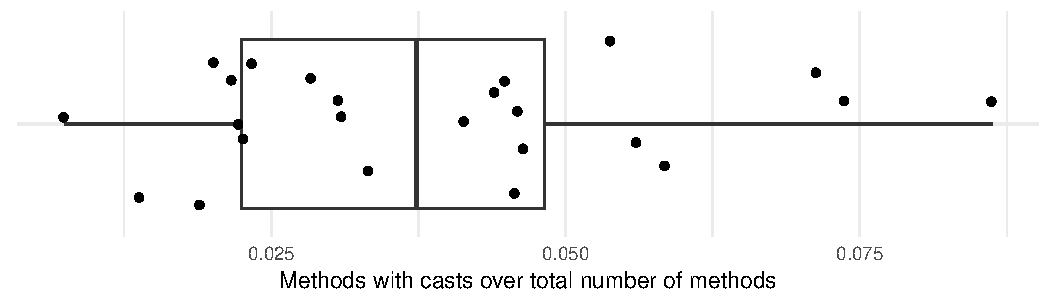
\includegraphics[width=\columnwidth]{stats-methodwcast.pdf}

All projects have less than $10\%$ of methods with at least a cast.
Overall, around a~$\castratio{}$ of methods contain at least one cast operation. 
This means there is a low density of casts.
Given the fact that generics were introduced \java{} 5, this can explain this low density.

Nevertheless, casts are still used.
We want to understand why there are casts instances (\ref{casts:rq2}) and how often the use cases that leads to casts are used (\ref{casts:rq3}).
The following sections give an answer to these questions.

% DONE: cut
% The query to gather this statistics is available online.\footnote{\url{https://gitlab.com/acuarica/java-cast-queries/blob/master/ql/stats.ql}}
% The \lang{R} script to further analyze the query results is available online as well.\footnote{\url{https://gitlab.com/acuarica/java-cast-queries/blob/master/analysis/stats.r}}

\section{Finding Casts Usage Patterns}
\label{sec:casts:methodology}

To answer both research questions
\ref{casts:rq2} (\emph{\crqB}) and \ref{casts:rq3} (\emph{\crqC}) we have used the \ql{} query language within the \lgtm{} service to look for cast instances.
As mentioned in section \ref{sec:casts:stats}, \ql{} treats primitive conversions as casts.
Thus, a preliminary step is to exclude them as cast instances.
The following \ql{} query shows how to retrieve all relevant cast expressions:

\begin{lstlisting}[style=ql,caption=\ql{} query to retrieve all relevant cast expressions.]
import java
from CastExpr ce where not (
ce.getExpr().getType() instanceof PrimitiveType and
ce.getTypeExpr().getType() instanceof PrimitiveType
) select ce
\end{lstlisting}

\tikzstyle{decision} = [diamond, aspect=2, draw, fill=blue!20, 
    text width=6em, text badly centered, node distance=3cm, inner sep=0pt]
\tikzstyle{block} = [rectangle, draw, fill=blue!20, 
    text width=7em, text centered, rounded corners, minimum height=2em]
\tikzstyle{block2} = [rectangle, draw, fill=blue!20, 
    text width=4.0em, text centered, rounded corners, minimum height=2em]
\tikzstyle{line} = [draw, -latex']
\tikzstyle{cloud} = [draw, ellipse,fill=red!20, node distance=3.1cm,
    minimum height=2.9em]

% \begin{wrapfigure}[h]
\begin{wrapfigure}{r}{7.6cm}
% \centering
\begin{tikzpicture}[node distance = 1.5cm, auto]
    % Place nodes
    \node [block] (run) {Run Query};
    \node [cloud, left of=run] (tags) {Tags};
    \node [cloud, right of=run] (patterns) {Patterns};
    \node [block, below of=run] (inspect) {Inspect Casts without Pattern};
    \node [decision, below of=inspect, node distance=1.6cm] (tag) {New Tag?};
    \node [decision, below of=tag, node distance=2.0cm] (pattern) {New Pattern?};
    \node [block2, left of=tag, node distance=3.1cm] (update-tags) {Update Tags};
    \node [block2, right of=pattern, node distance=3.1cm] (update-pattern) {Update Patterns};
    % \node [decision, below of=evaluate] (decide) {is best candidate better?};
    \node [block, below of=pattern, node distance=1.6cm] (stop) {Stop};
    % Draw edges
    \path [line] (run) -- (inspect);
    % \path [line] (inspect) -- (evaluate);
    \path [line] (inspect) -- (tag);
    % \path [line] (inspect) -- (pattern);
    \path [line] (tag) -- node [near start] {yes} (update-tags);
    \path [line] (pattern) -- node [near start] {yes} (update-pattern);
    \path [line] (update-tags) -- (tags);
    \path [line] (update-pattern) -- (patterns);
    \path [line] (tag) -- node {no}(pattern);
    \path [line] (pattern) -- node {no}(stop);
    \path [line,dashed] (tags) -- (run);
    \path [line,dashed] (patterns) -- (run);
\end{tikzpicture}
\caption{Process to discover cast tags and patterns.} \label{fig:process}
\end{wrapfigure}


Figure~\ref{fig:process} depicts our methodology.
We have used this initial result as a starting point for our analysis.
Afterwards, we select a random sample for manual inspection.
We manually inspected the mentioned casts trying to understand why and how they were used.

By manually inspecting several casts instances, we observe that certain characteristics appear often, \eg{}, a cast in a overridden method, or a cast guarded by an \code{instanceof}.
We then \emph{tag} cast instances based on these observations.
We implement a \ql{} predicate that detects them and proceed to refine our query with this new tag predicate.
% The table of tags is presented in table~\ref{table:tags}.
After a new tag is added, the query is run again to iterate over the new results.

% DONE: Remove randomly.
% Whenever we observe that those tags do not appear randomly,
Whenever we detect that those tags appear often,
we further inspect the source code to check that is indeed a pattern.
We have formalize the structure of each pattern as a \ql{} predicate based on those tags.
Similarly with tags, after a new pattern is added, the query is run again to inspect the casts without pattern.
To sum up, our methodology iterates over the results until no \emph{more} patterns can be detected.
% These patterns are presented in the following section.
The final \ql{} query is available online.\footnote{\url{https://gitlab.com/acuarica/java-cast-queries/blob/master/ql/obs.ql}}


% DONE: What about patterns we can't write queries for?
\subsection*{Manual Categorization of Patterns}

Some code patterns might be too difficult to express in terms of \ql{} queries.
This situation arises when the knowledge to determine the pattern is outside the source code,
\eg, in configuration files or library call sites.
Thus, in those cases we can only acknowledge that a pattern exists, but not how recurrent it is.

% \begin{table*}[t!]
% \centering
% \caption{Cast tags used to discover cast patterns.}
% \label{table:tags}
% \input{table-tags.inc}
% \end{table*}